\documentclass{math201}
\usepackage{hyperref}
\usepackage{bookmark}
\usepackage{minted}

% =============================================
% Part 0 信息
% =============================================

\mathsetup{
  % 学生姓名
  student = {某同学},
  % 学号
  student-id = {2021xxxx},
  % 院系
  experiment = {实验四 串口通信实验},
  % 专业年级
  discipline = {集成电路设计与集成系统},
  % 日期
  date = {2024 年 4 月 1 日},
}

\begin{document}

% =============================================
% Part 1  封面
% =============================================

\makecover

% =============================================
% Part 2 主文档
% =============================================

\section{实验要求}

\begin{enumerate}
  \item 运行例程实验5 USART指令控制LED灯,观察实验现象
  \item 看懂源程序
  \item 修改源程序,当输入的最后一个数字是奇数的时候蜂鸣器中响一声,偶数的时候蜂鸣器响两声(两声之间的间隔自己确定)
  \item 撰写实验报告、把修改的程序截图、实验现象的裁图或者图片整理到报告中
\end{enumerate}

\section{实验内容及结果}

\subsection{编写代码}

然后修改\textbf{main.c},对串口输入的数字进行处理,将其转换为整数,判断奇偶性,控制蜂鸣器。

\begin{enumerate}
  \item \textbf{初始化设置}:
    - 初始化RGB彩灯和USART通信模块,确保硬件正常工作。
    - 设置USART通信参数为115200波特率,8位数据位,无校验位,1位停止位。

  \item \textbf{打印指令提示信息}:
    - 在主函数中,调用\texttt{Show\_Message()}函数,打印出指令输入的提示信息。
    - 用户被要求输入数字字符。
  
  \item \textbf{接收字符指令}:
    - 程序等待用户输入一个数字字符。
    - 通过\texttt{getchar()}获取字符,并打印接收到的字符。

  \item \textbf{判断奇偶性}:
    - 将接收到的字符转换为整数。
    - 判断该整数是奇数还是偶数。
    - 如果是偶数,蜂鸣器响两声;如果是奇数,蜂鸣器响一声。

  \item \textbf{延时函数}:
    - 提供了一个简单的延时函数,用于实现延时操作。
\end{enumerate}

\inputminted[
    frame=lines,
    framesep=2mm,
    baselinestretch=1.2,
    fontsize=\small,
    linenos
]{C++}{code/main.c}

\subsection{下载运行}

使用 \texttt{FlyMCU.exe} 下载程序到 STM32 开发版上,观察实验现象。

\subsection{实验现象}

\begin{figure}[H]
  \centering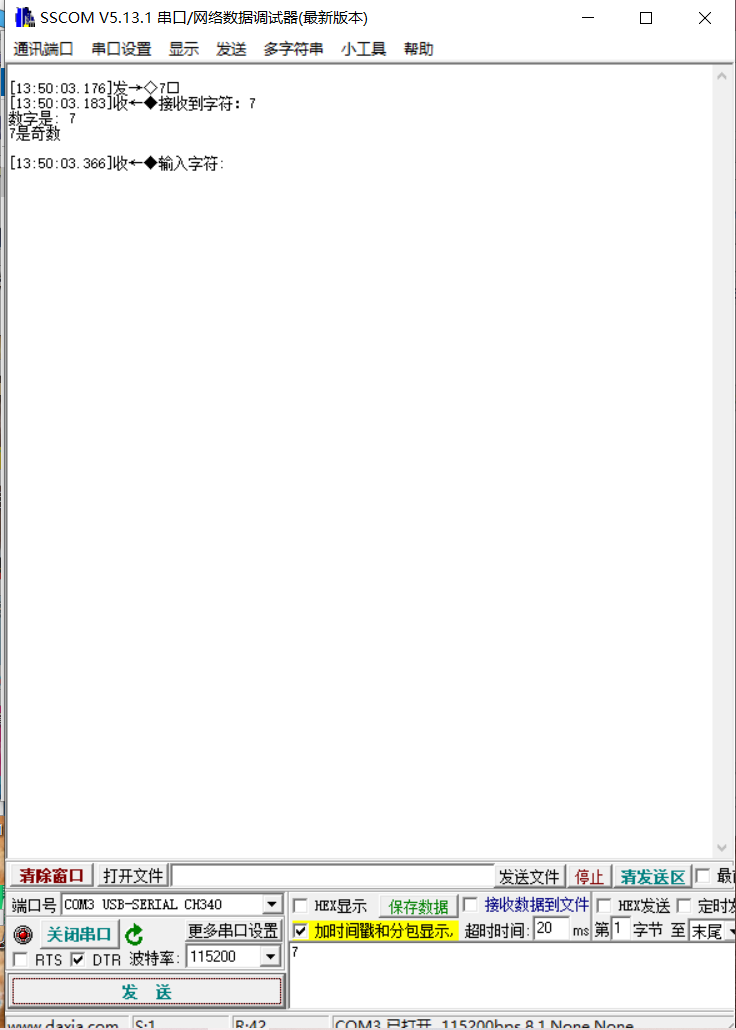
\includegraphics[width=0.6\linewidth]{result.jpg}
  \caption{奇偶性判断}      
\end{figure}

\section{实验小结}

通过本次实验,我学会了如何使用串口通信控制 STM32 开发板上的蜂鸣器,实现了对输入数字奇偶性的判断,并控制蜂鸣器的响声。

\end{document}
